
%\documentclass[10pt,onecolumn,twoside]{IEEEtran} %!PN
%  \documentclass[10pt,twocolumn,twoside]{IEEEtran} %!PN
% \documentclass[12pt,onecolumn,twoside,draft]{IEEEtran} %!PN
%\documentclass[conference]{IEEEtran} %!PN
%\documentclass[conference]{IEEEtran}

\documentclass{sig-alternate}
%\documentclass{article}
%\usepackage{spconf} %ICME conf style

\usepackage{multirow}
\usepackage{amsfonts}
\usepackage{epsfig}
\usepackage{amsmath}
\usepackage{amssymb}
%%\usepackage[nolist]{acronym}
\usepackage[acronym]{glossaries}
\newcommand\acro[2]{\newacronym{#1}{#1}{#2}}
\newcommand\acroAlwaysShort[1]{\newglossaryentry{#1}{type=\acronymtype, name={#1}, description={#1}, text={#1}, first={#1}, plural={#1s}, firstplural={#1s}}}
\newcommand\acroShortSurname[2]{\newglossaryentry{#1}{type=\acronymtype, name={#2}, description={#2}, text={#2}, first={#2}, plural={#2s}, firstplural={#2s}}}
\newcommand\ac[1]{\gls{#1}}
\newcommand\acp[1]{\glspl{#1}}
\newcommand\acs[1]{\glsname{#1}}
\newcommand\acl[1]{\glsentrylong{#1}}

\acro{FoV}{Field of View}
\acro{ABR}{adaptive bit-rate}
\acro{DASH}{Dynamic Adaptive Streaming over HTTP}
\acro{CDN}{content delivery network}
\acro{CDF}{cumulative density function}
\acro{HMD}{Head-Mounted Display}
\acro{PDF}{probability density function}
\acro{RTP}{real-time protocol}
\acro{VR}{Virtual Reality}
\acro{QoE}{Quality of Experience}
\acro{VQM}{Video Quality Metric}
\acro{ILP}{integer linear program}
\acro{HDTV}{high definition television}
\acro{UGC}{User-Generated Content}
\acro{MPD}{Media Presentation Description}
\acro{PSNR}{Peak Signal Noise to Ratio}
\acro{GPU}{graphics processing unit}
\acro{CPU}{central processing unit}
\acro{MS-SSIM}{Multiscale - Structural Similarity}
\acro{API}{Application Programming Interface}
\acro{QEC}{Quality Emphasis Center}
\newglossaryentry{RoI}{type=\acronymtype, name={RoI}, description={RoI}, text={RoI}, first={Region of Interest~(RoI)}, plural={RoI}, firstplural={Regions of Interest~(RoI)}}
\acro{VM}{Virtual Machine}
\acro{SVC}{Scalable Video Coding}
\acro{GOP}{Group of Picture}
\acro{PMU}{Performance Monitoring Unit}
\acro{LAN}{Local Area Network}
\acro{AI}{Artificial Intelligence}
\acro{3D}{Three Dimentional}
\acro{OS}{Operating System}
\newglossaryentry{fps}{type=\acronymtype, name={fps}, description={frame per second}, text={frame per second}, first={frame per second~(fps)}, plural={fps}, firstplural={frames per second~(fps)}}
\newglossaryentry{p}{type=\acronymtype, name={p}, description={p}, text={~pixel}, first={~pixel (p)}, plural={p}, firstplural={~pixels (p)}}
\newglossaryentry{s}{type=\acronymtype, name={s}, description={s},
text={second}, first={~second~(s)}, plural={s}, firstplural={~seconds~(s)}}
\acroAlwaysShort{TCP}
\acroAlwaysShort{HTTP}
\acroAlwaysShort{MPEG}
\acro{RTT}{Round-Trip Time}
\acro{AVC}{Advanced Video Coding}
\acro{HEVC}{High Efficiency Video Coding}
\acro{ISO}{International Organization for Standardization}
%\acro{ISOBMFF}{\ac{ISO} base media file format}
\newglossaryentry{ISOBMFF}{type=\acronymtype, name={ISOBMFF}, description={International Organization for Standardization base media file format}, text={International Organization for Standardization base media file format}, first={International Organization for Standardization base media file format ISO/IEC 14496-12 (ISO BMFF)}, plural={ISO BMFFs}, firstplural={International Organization for Standardization base media file formats (ISO BMFFs)}}
\acro{MTU}{Maximum Transmission Unit}
\acro{AQM}{Active Queue Management}
\acro{I}{intra-predicted}
\acro{P}{inter-predicted}
\acro{B}{bidirectional}
\acro{VQMT}{Video Quality Measurement Tool}
\acro{EPFL}{Ecole Polytechnique F\'{e}d\'{e}rale de Lausanne}
\acroShortSurname{YUV}{YUV}
\acroShortSurname{RGB}{R'G'B'}
\acro{MSE}{Mean Square Error}
\acro{CMSE}{Commulative Mean Square Error}
 % acronymes + associated packages  are defined in the acronymes.tex file
\usepackage[english]{babel}
%\usepackage{cite}
\usepackage[numbers,sort]{natbib}
\renewcommand\citet[1]{\citeauthor{#1}~\cite{#1}} % redefine the \citet command to add a ~ space between authors and []
\usepackage{color}
\usepackage[dvipsnames]{xcolor}
\usepackage{stfloats}
%\usepackage{pst-gantt}
% \usepackage{algorithm}
% \usepackage{algorithmic}
\usepackage[linesnumbered,ruled,vlined,boxed,commentsnumbered]{algorithm2e}
\usepackage[noend]{algorithmic}
\usepackage{float}
\algsetup{linenosize=\tiny}
%\usepackage{caption}
%\usepackage{subcaption}
\usepackage[caption=false]{subfig}
\usepackage{pgfplots}
\usepackage{booktabs}
\usepackage{listings}
\usepackage[hidelinks]{hyperref}
%\usetikzlibrary{plotmarks}
\usetikzlibrary{shapes,positioning,3d,calc}
\usetikzlibrary{decorations,decorations.pathmorphing}
\usetikzlibrary{external}
\newcommand{\externaldirectory}{latex.out/}
\tikzexternalize[prefix=\externaldirectory]
\tikzexternalize % activate!
\tikzexternaldisable
\usepackage{wrapfig}
\usepackage{enumitem}
\usepackage{url}
\usepackage{etoolbox}

\lstset{%
  backgroundcolor=\color{gray!25},
  basicstyle=\sffamily \scriptsize,
  breaklines=true
}

%SI Units
\usepackage{siunitx}
\sisetup{detect-all}

%math tools
\usepackage{mathtools}
\usepackage{stmaryrd}
\usepackage{mathrsfs}
\usepackage{amssymb}
%Some math declarations
\DeclarePairedDelimiter{\ceil}{\lceil}{\rceil}
\DeclarePairedDelimiter{\parenthesis}{(}{)}
\DeclarePairedDelimiter{\set}{\{}{\}}
\DeclarePairedDelimiter{\norm}{|}{|}
\DeclarePairedDelimiter{\integerInterval}{\llbracket}{\rrbracket}
\DeclareMathOperator*{\minimize}{minimize}

%Some symbols definitions
\newcommand{\packetset}{\mathcal P}
\newcommand{\frameset}{\mathcal F}
\newcommand{\packetsubset}{\mathcal P'}
\newcommand{\framesubset}{\mathcal F'}


% fix the issue of white character in acronym package
\usepackage{etoolbox}
\makeatletter
\patchcmd\@acf{\hskip\z@}{}{}{}
\patchcmd\@acf{\hskip\z@}{}{}{}
\makeatother


\usepackage{pgfplotstable}
\pgfplotsset{compat=1.8}


\newbool{NotesActivated}
\booltrue{NotesActivated}  %comment this line to remove all user comments

%include some macro specific for this paper
\newcommand\algoFontSize{8}
\newcommand{\noteGS}[1] {\ifbool{NotesActivated}{\color{red}\{\textbf{GS:}\textit{{#1}}\}\color{black}}{}}
\newcommand{\noteXC}[1] {\ifbool{NotesActivated}{\color{YellowOrange}\{\textbf{XC:}\textit{{#1}}\}\color{black}}{}}
\newcommand{\noteFB}[1] {\ifbool{NotesActivated}{\color{OliveGreen}\{\textbf{FB:}\textit{{#1}}\}\color{black}}{}}
\newcommand{\noteGA}[1] {\ifbool{NotesActivated}{\color{Blue}\{\textbf{GA:}\textit{{#1}}\}\color{black}}{}}
\newcommand{\noteGT}[1] {\ifbool{NotesActivated}{\color{Salmon}\{\textbf{GT:}\textit{{#1}}\}\color{black}}{}}
\newcommand\newpara[1]{\vspace{3pt}\noindent\textbf{#1}.\hspace{0.15cm}}
\newcommand\newsubpara[1]{\vspace{0.15cm}\noindent\textit{#1}.\hspace{0.15cm}}

%Define names of the Estimation Functions
\newcommand{\setPositive}{ % STYLE
   \text{\bf{\scriptsize+}}
}
\newcommand{\setNegative}{ % STYLE
   %\mathbb{\tiny-}
   \text{\large-}
}
\newcommand\constantParam[1]{
    {\scriptsize \{ #1 \}}
}


%\newcommand\R{\emph{Random}}
%\newcommand\TR{\emph{Type}}
%\newcommand\DR{\emph{Dependencies}}
%\newcommand\SP{\emph{DropSmall}}
%\newcommand\DSP{\emph{DepDropSmall}}
%\newcommand\DSM{\emph{DepDropBig}}
%\newcommand\DTSM{\emph{HybridDropBig}}
%\newcommand\DTSP{\emph{HybridDropSmall}}


\newcommand {\otoprule }{\midrule [\heavyrulewidth]}

\title{Adaptive Delivery of Navigable 360-Degree Videos}

\tolerance=1
\emergencystretch=\maxdimen
\hyphenpenalty=10000
\hbadness=10000

\floatstyle{ruled}
\newfloat{ilp}{ht}{aux}
\floatname{ilp}{Integer Linear Program}


\newbool{doubleBlinded}
\booltrue{doubleBlinded}  %comment this line to remove all user comments

\makeatletter
%\def\@name{ \ifdoubleBlinded \phantom{ \fi \emph{Xavier Corbillon$^{\star}$ \quad Florian Boyrivent$^{\star}$
%\quad Gr\'{e}goire Asselin\,De\,Williencourt$^{\star}$} \ifdoubleBlinded } \fi \\ \ifdoubleBlinded \phantom{ \emph{Gwendal
%Simon$^{\star}$ \quad G\'{e}raldine Texier$^{\star}$ \quad Jacob
%Chakareski$^{\dagger}$}\ifdoubleBlinded } \fi}
%
%\address{\ifdoubleBlinded \phantom{ \fi $^{\star}$ T\'{e}l\'{e}com Bretagne / IRISA, France \ifdoubleBlinded } \#$144$ \phantom{ \fi\quad
%$^{\dagger}$ University of Alabama, USA \ifdoubleBlinded } \fi}

\ifdoubleBlinded
\numberofauthors{1}
\else
\numberofauthors{3}
\fi

\author{ 
\alignauthor
\ifdoubleBlinded
        Paper ID 
\else
  Xavier Corbillon\\
  \affaddr{T\'{e}l\'{e}com Bretagne, IRISA, France}% \\
\alignauthor
  Alisa Devlic\\
  \affaddr{T\'{e}l\'{e}com Bretagne, IRISA, France}% \\
\alignauthor
  Gwendal Simon\\
  \affaddr{T\'{e}l\'{e}com Bretagne, IRISA, France}%\\
\fi
}



\makeatother

%\pgfdeclareimage[width=3cm]{gamer}{plots/game-controller-icon-614x460.png}
%\pgfdeclareimage[width=1.6cm]{tv}{plots/1411044172_PixelKit_tv_icon.png}
%\pgfdeclareimage[width=0.8cm]{rack}{plots/1411044156_PixelKit_network_icon.png}


\begin{document}
%\ninept

\maketitle

\begin{abstract}
Here is the Abstract.


\end{abstract}
%%% Local Variables:
%%% mode: latex
%%% TeX-master: "paper"
%%% End:


\section{Introduction}
\label{sec:introduction}

\subsection{Context and Motivations}

The popularity of interactive 360-degree video systems (also known as immersive omnidirectional video) 
has grown with the advent of both capturing systems
(including catadioptric optical systems and multi-camera with stitching systems) and video
consumption systems (including head-mounted display and interactive HTML5 video players).
However, the delivery of 360-degree video content, from the servers of the content providers
to the end-users,
is still a challenge. Head-mounted devices display two videos (one per
eye), each of them with a high resolution (typically $1080\times 1200$ for state-of-the-art devices)
and a high frame rate. Both videos, which correspond to the \ac{FoV} on both eyes, are extracted
from a wider spherical video with a resolution that is three to four times larger.

None of the current solutions for the delivery of 360-degree videos is entirely satisfactory. Sending only 
the \ac{FoV} videos is the least bandwidth-hungry implementation. It requires however the server to 
compute the \ac{FoV} from the spherical video for each end-user. Moreover, it does not enable fast
navigation within the scene: When the client changes the 
\ac{FoV}, the device cannot immediately display any video because it does not have information on the other
parts of the full spherical video. The device has to notify the server and to wait for the reception of the 
newly adjusted \ac{FoV} videos. Another delivery implementation is to send the full spherical video 
and to let the device
extract the \ac{FoV} videos. This solution enables fast navigation but the bandwidth requirements are 
significant.

We explore in this paper a solution where the server offers multiple \emph{versions} of the same 
360-degree  video. Each version is characterized by an \emph{angle of vision}. It contains the full spherical 
video with an emphasis on the given angle of vision, \textit{i.e.},
the part of the video that is in front of the angle of vision is at the highest quality and the video quality 
degrades for the other parts. The client device chooses the video version according to the eye attention 
such that the 
the front view of the video version is close to the \ac{FoV} videos. Thus, the \ac{FoV} extraction is done
from the high quality spherical video. When the end-user changes the 
\ac{FoV}, the device can always extract a \ac{FoV} video (sometimes from a low quality part of the 
full video) until it switches to a new video version that better suits the new visual attention.

\subsection{Limitations of Previous Work}

The principle of differentiated video quality in the delivery of omnidirectional videos has been sketched 
in a recent short paper by~\citet{ochi_live_2015}. Their proposal is based on the idea of video
tiling, which has been implemented for navigable panorama 
video~\cite{sanchez_compressed_2015,wang_mixing_2014,gaddam_tiling_2015}: The panorama video 
is cut into independent \emph{tiles} (typically $8\times 8$) and the server offers several
video qualities for each tile. The client selects the quality of each tile according to the eye attention. This
solution has the same advantages of our proposal, since it reduces the overall bandwidth by emphasizing
the video quality only for the parts that are actually watched, at the price of transient lower quality just after
brutal navigation events. However, this solution does not take into account the characteristics of 360-degree
videos. A spherical video can be mapped into an \emph{equirectangular} video without losing any information
for the extraction of \ac{FoV}, but the pixels at the poles are over-sampled (the number of pixels
used in the rectangle to depict a pixel into the sphere is higher at the pole than in the equator). 
This characteristic is known to degrade the
performance of traditional video encoders~\cite{wojciechowski_h.264_2006,yu_framework_2015}. It also 
makes equirectangular tiling less relevant.

The mapping of spherical videos into 2D video is a projection that generates distortion on the resulting
full 2D video, but some projections enable \ac{FoV} extraction without information loss. It is typically the case of 
projections on \emph{cube map}~\cite{Ng2005} and 
\emph{rhombic dodecahedron}~\cite{fu_rhombic_2009}. The previous work regarding mapping into these
geometrical layouts has focused on enabling efficient implementation of signal processing 
functions~\cite{kazhdan_metric-aware_2010} and improving the video encoding~\cite{tosic_low_2009}. 
However, to the best of our knowledge, the 
question of differentiated quality on the different faces of the layouts has not been studied so far.

Finally, a major content provider of 360-degree videos has recently released details about the 
implementation of its delivery platform~\cite{facebook}. The depicted system is based on the same
main idea as our proposal, where up to 30 versions of the same video are available according to angles
of vision. This description corroborates that, from an industrial perspective, the extra-cost of
generating and storing multiple versions of the same video is relevant with respect to the bandwidth
savings. The authors use a mapping of the spherical videos into a pyramid where the base is the front
view and the peak is behind. Yet, this mapping under-samples some pixels, which results in 
information loss and distorted extraction of \ac{FoV} videos.

\subsection{Our Contributions}

In this paper, we present a system for navigable 360-degree video delivery. Our focus is
about the mapping of spherical videos into geometrical layouts with differentiated qualities
with respect of angle of visions. Our contribution is twofold:
\begin{itemize}
\item We introduce a tool (released on open source in a public repository\footnote{url is hidden for blind
preservation.}) that enables the mapping from a spherical video
into any geometrical layout (and vice versa). The tool has two main features: it enables differentiated
quality for different parts of the 2D video with respect to the geometrical layouts, and it extracts the 
\ac{FoV} videos from any point in the sphere. With this tool, the scientific community will be able to 
study the mapping of spherical videos for the delivery of 360-videos and the implementation of delivery 
solutions.
\item We provide a comprehensive comparison of the different quality-differentiated 
mappings regarding
the bit-rate of the resulting videos, the quality of the extracted \ac{FoV} videos, and the capacity to
implement smooth navigation. Thus, we address most of
the questions raised by~\citet{facebook}: which layout provides the best trade-off between bit-rate and
quality, how many video versions should be offered by the server, and what tile quality implementation 
enables the smoothest navigation.
\end{itemize}

In this short paper, we restrict our study to essentials, and we provide only our main findings based on a 
sample of the results. \textit{Here are our findings...}




%%% Local Variables:
%%% mode: latex
%%% TeX-master: "paper"
%%% End:


% =============
\section{Navigable 360-degree Video Delivery}

We provider in this Section the background for our study.
First, we depict the overall architecture of the delivery system that we envisioned.
Then, we recall the main geometrical mappings that exist for 360-degree videos.

\subsection{Global Delivery Architecture}

We introduce here the main principles of the delivery architecture and we let for future 
work the complete description and the performance evaluation.

\begin{figure}[h]
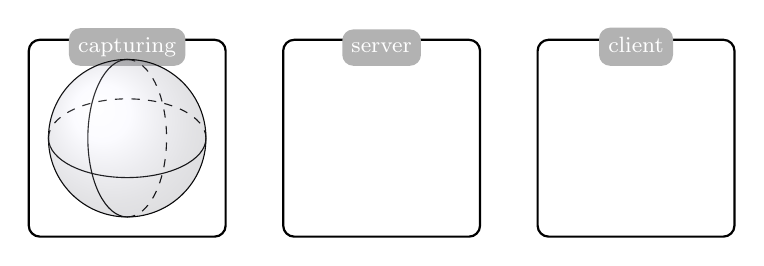
\begin{tikzpicture}

\tikzset{
     element/.style={
     	rounded corners,
     	rectangle,
  	 	thick,
  	 	draw=black,
  	 	minimum height=2.5cm,minimum width=2.5cm
     }
}

\tikzset{
	elementtitle/.style={
		rectangle,
		rounded corners,
		fill=gray!60,
		font=\footnotesize,
		text=white,
		anchor=north
	}
}

\tikzset{
	spherical/.pic={
		\draw (-1,0) arc (180:360:1cm and 0.5cm);
	    \draw[dashed] (-1,0) arc (180:0:1cm and 0.5cm);
    	\draw (0,1) arc (90:270:0.5cm and 1cm);
    	\draw[dashed] (0,1) arc (90:-90:0.5cm and 1cm);
    	\draw (0,0) circle (1cm);
    	\shade[ball color=blue!10!white,opacity=0.20] (0,0) circle (1cm);
    }
}
		
\def\ecart{20pt}



% capturing system
\node[element] (0,0) (capturing) {};
\node[elementtitle, above=-10pt of capturing] {capturing};
\draw (capturing) pic {spherical};

% server
\node[element,right=\ecart of capturing] (server) {};
\node[elementtitle, above=-10pt of server] {\vphantom{pt}server};

% client
\node[element,right=\ecart of server] (client) {};
\node[elementtitle, above=-10pt of client] {\vphantom{pt}client};


\end{tikzpicture}
\caption{Global architecture of the navigable 360-degree video delivery system}
\end{figure}


\subsection{Mapping of Spherical Videos}

\subsubsection{Equirectangular}

\subsubsection{Cube Maps}

\subsubsection{Pyramid}

\subsubsection{Rhombic Dodecahedron}

\section{Quality-Differentiated Mapping Evaluation}

\subsection{Evaluation Platform}

\subsection{Results}

\section{Discussion and Conclusion}

\newpage
%%%%%%%%%%%%%%%%%%%%%%%%%%%%%%%
%\bibliographystyle{IEEEtran}
%\bibliographystyle{IEEEbib}
\bibliographystyle{abbrvnat}  
%\bibliographystyle{abbrv}  
\bibliography{biblio}

\end{document}

